\section{Prototypes}
This section will describe the setup of the prototypes developed during this project.

\subsection{Prototype \#1}
\label{sec:implementation:prototypes:prototype1}
The first prototype was an Android phone application that showed the location of the user, the direction the phone was pointing, and the devices that were being pointed at.
The application used a $10 \times 10$ grid to simulate a square room in which the user and the devices to be controlled were located.
A set of imaginary devices was hardcoded into the application with fixed positions and the grid would look like the one shown in \Cref{table/prototype-grid}.
The user is positioned in the center at (5,5) by default. This position can be changed by using the \texttt{Up}, \texttt{Down}, \texttt{Left} and \texttt{Right} buttons.
When the user's direction changes a list of devices being pointed at is acquired by calculating the angle between the user's position and the position of each device.
The direction is found using magnetic fields such that $0$ is north, $-90$ is west, $90$ is east, etc. 
The angle between each smart device and the user is calculated finding the inverse tangent (arctangent) and then converting from radians to degrees such that we get:
\begin{equation}
\var{angle} = 180 / \pi * \arctan(\var{user.y} - \var{device.y} / \var{user.x} - \var{device.x})
\end{equation}
where \var{user.x} and \var{user.y} are the $x$ and $y$ coordinates of the user and likewise for the device.
A screenshot of this application is shown in \Cref{fig:prototype1-app-screenshots}.


\begin{table} % Thalley: Måske lave om et et Tikz coordinatsystem i stedet for? Fylder unødvendigt meget imo. 
    \centering
    \scriptsize
    \begin{TAB}(e,1cm,1cm){|c:c:c:c:c:c:c:c:c:c|}{|c:c:c:c:c:c:c:c:c:c|}
     &  &  &  &  &  &  &  &  & Stereo \\
     &  &  &  &  &  &  &  &  &  \\
     &  &  &  &  &  & \begin{tabular}[c]{@{}l@{}}Coffee\\ Maker\end{tabular} &  &  &  \\ 
     &  &  &  &  &  &  &  &  &  \\ 
    \begin{tabular}[c]{@{}l@{}}Garage\\ Door\end{tabular} &  &  &  &  &  &  &  &  &  \\ 
     &  & Lamp 2 &  &  &  &  &  &  &  \\
     &  &  &  &  &  &  &  &  &  \\ 
     &  &  &  &  &  &  &  &  &  \\ 
     &  &  &  &  &  &  &  &  &  \\ 
    Lamp 1 &  &  &  &  & TV &  &  &  &  \\
    \end{TAB}    
    \caption{Grid showing the position of devices. Lamp 1 is located at (0,0) and Stereo is located at (9,9)}
    \label{table/prototype-grid}
\end{table}

\begin{figure}%
    \centering
    \subfloat{
        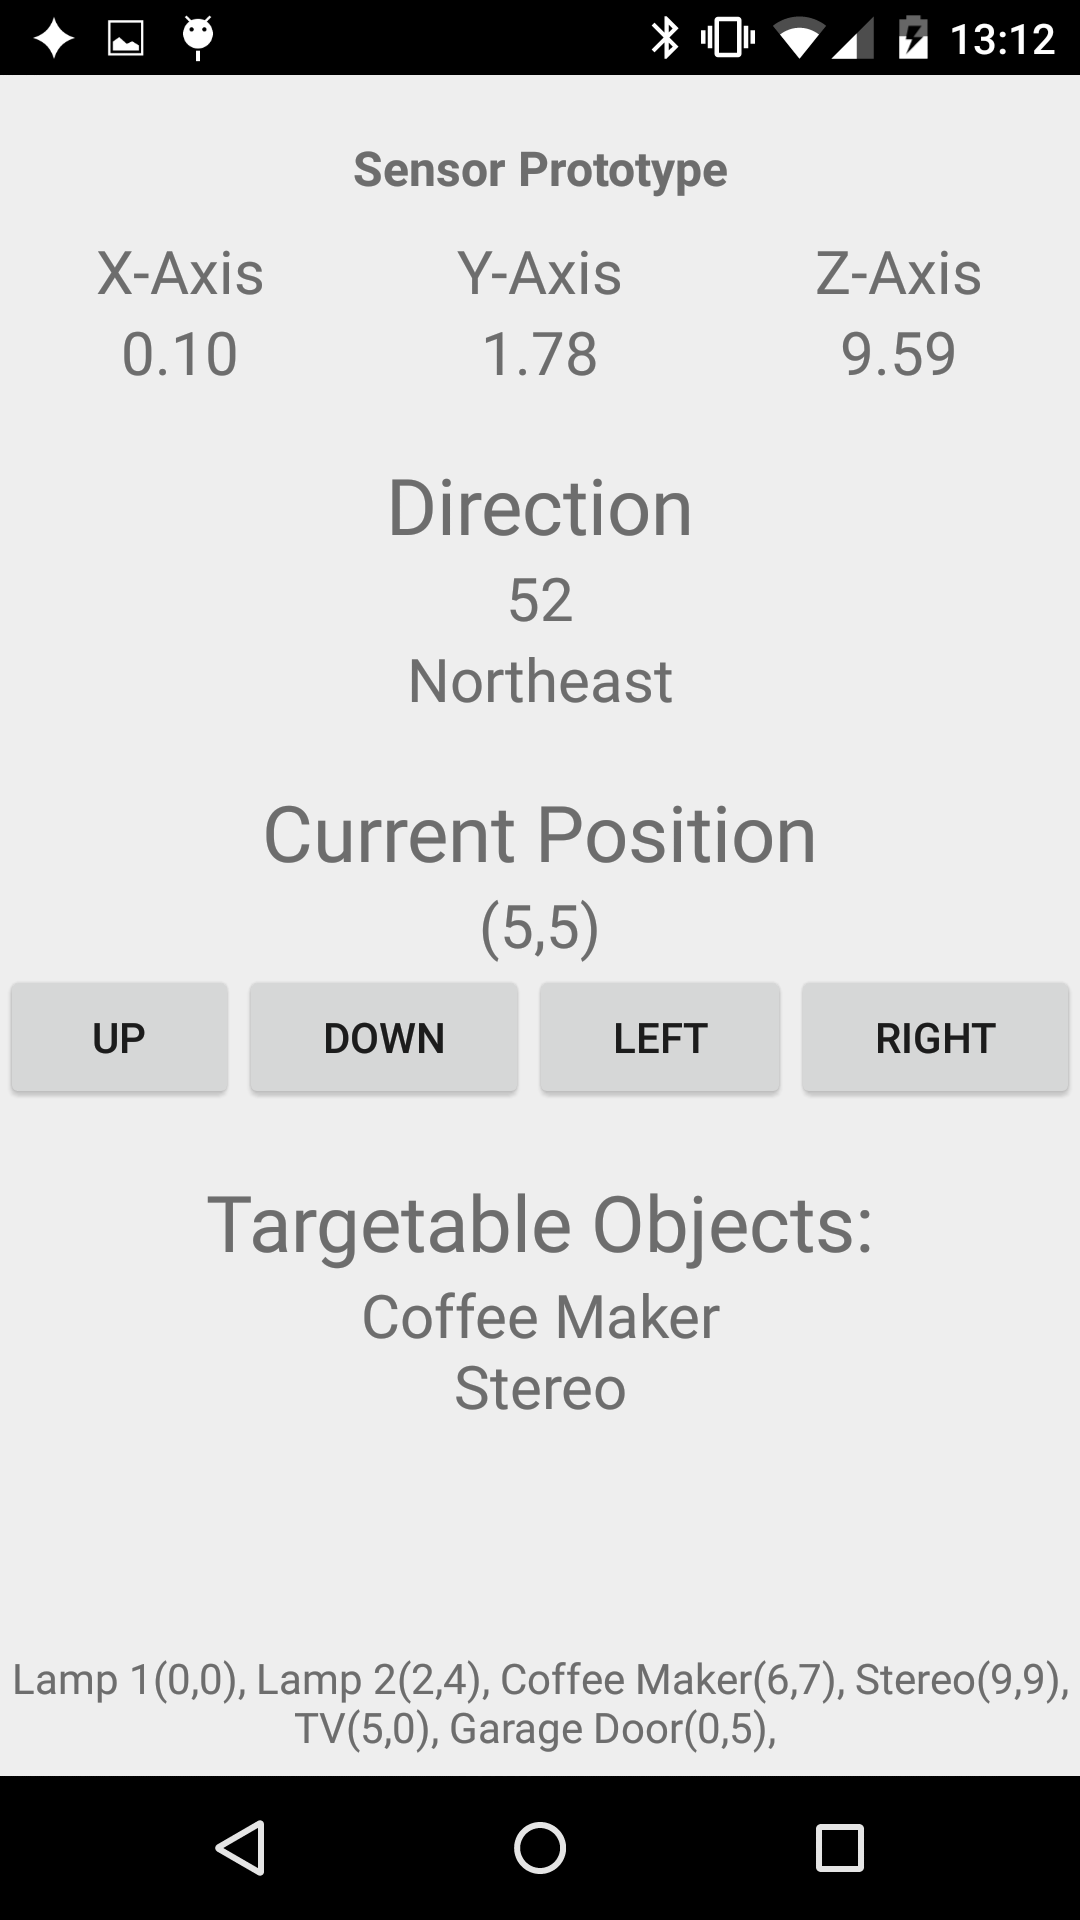
\includegraphics[width=0.3\textwidth]{images/Prototype1_Android_1.png}
    }
    \subfloat{
        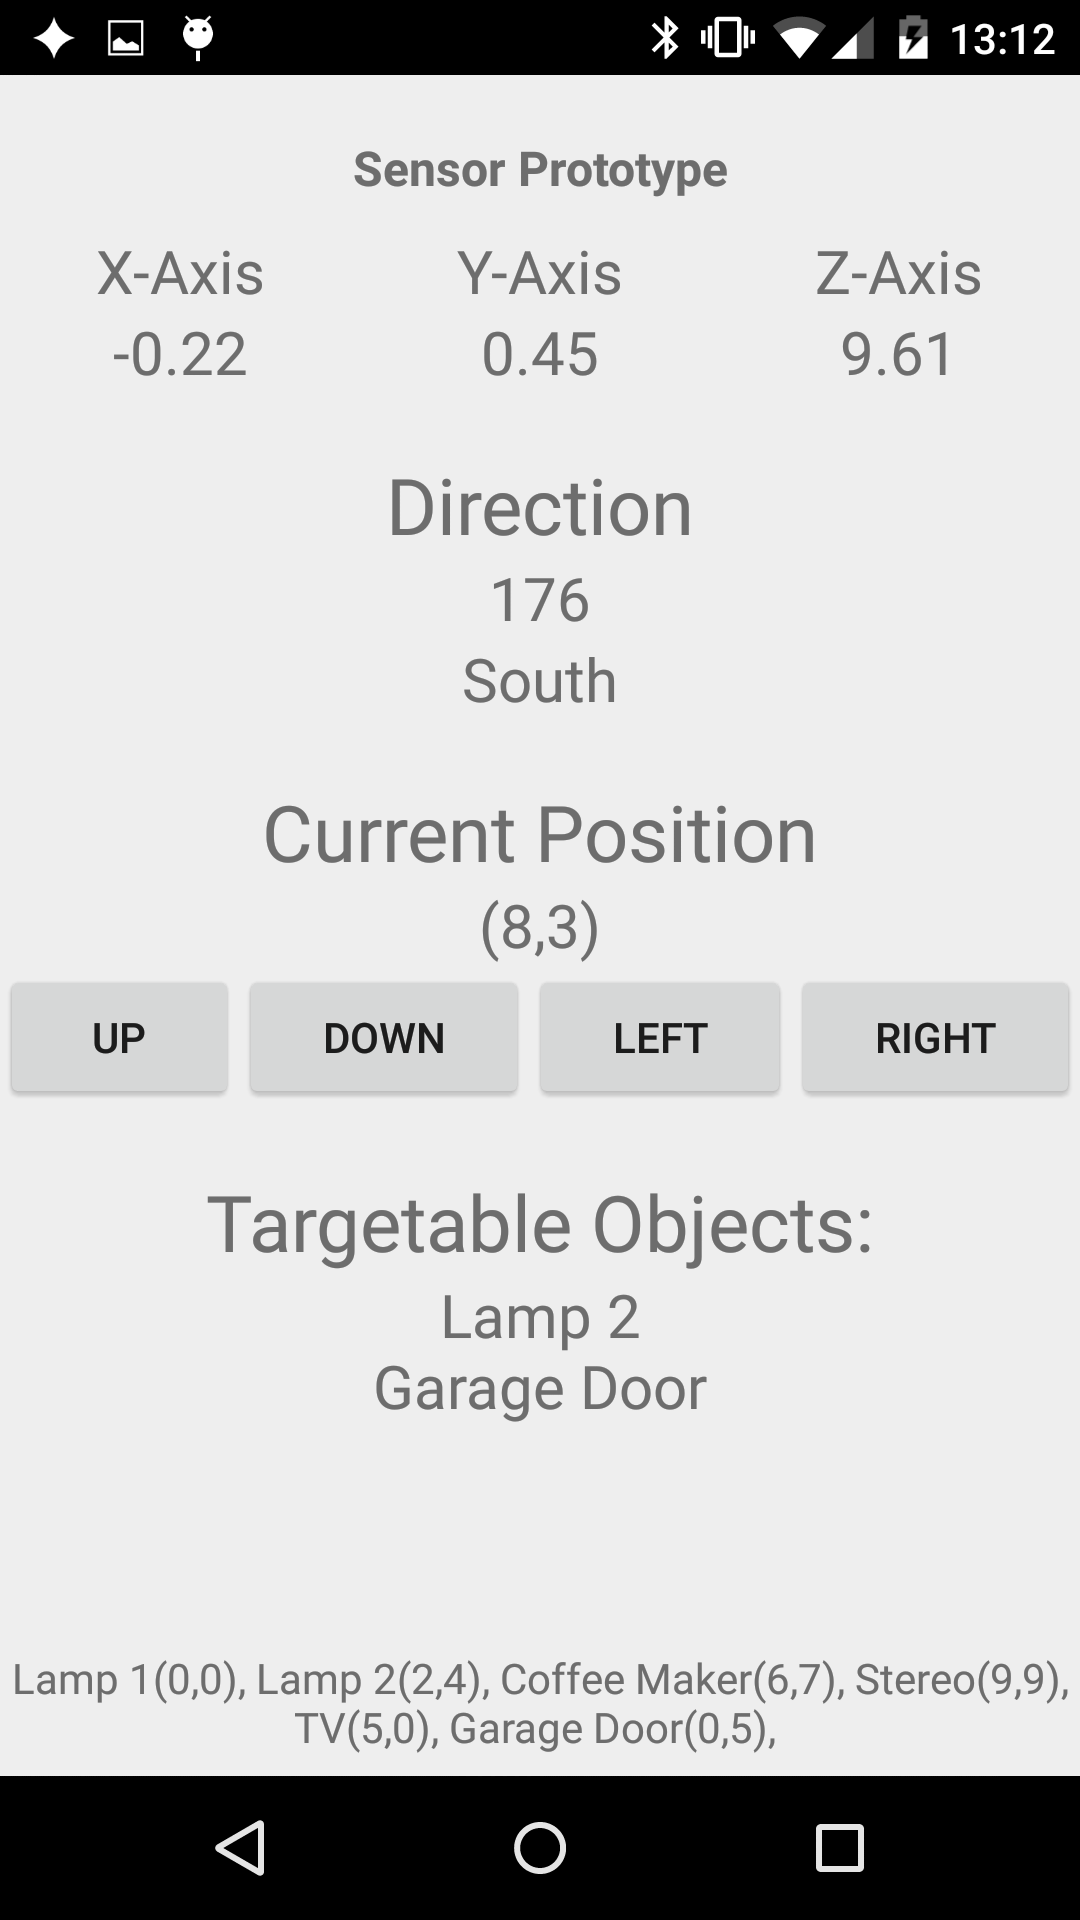
\includegraphics[width=0.3\textwidth]{images/Prototype1_Android_2.png}
    }
    \caption{Screenshots of the first prototype.}
    \label{fig:prototype1-app-screenshots}
\end{figure}


\subsection{Prototype \#2}
\label{sec:implementation:prototypes:prototype2}

The second prototype consisted of an iOS application similar to the Android application described in section \ref{sec:implementation:prototypes:prototype1} and a server that represented two controllable lamps.
The platform was changed from Android to iOS because the application would later use Estimote beacons and there was no Android Indoor Location SDK available for this. 

\subsubsection*{Major Changes}
\begin{itemize}
\item Introduction of a server for the application to interact with.
\item Switched platform from Android to iOS.
\end{itemize}

In this prototype the room is still represented as a grid and the user is placed in the center of the grid, however the user is unable to change position.
This is because the first prototype showcased the idea of pointing at devices from different locations sufficiently and the next step would be to use the actual location of a user using Estimote beacons.
As shown in \Cref{fig:prototype2-app-screenshots} the user can see his direction as an angle between himself and north.
Devices are represented as orange dots and if the user points towards one of them two buttons will appear that allow the user to interact with the device by either turning it \texttt{on} or \texttt{off}.
When the user turns a device on or off it will be reflected on the server where a corresponding box will have the color \texttt{green} when turned on and \texttt{red} when turned off as shown in \Cref{fig:prototype2-server-screenshot}.

\begin{figure}%
    \centering
    \subfloat{
        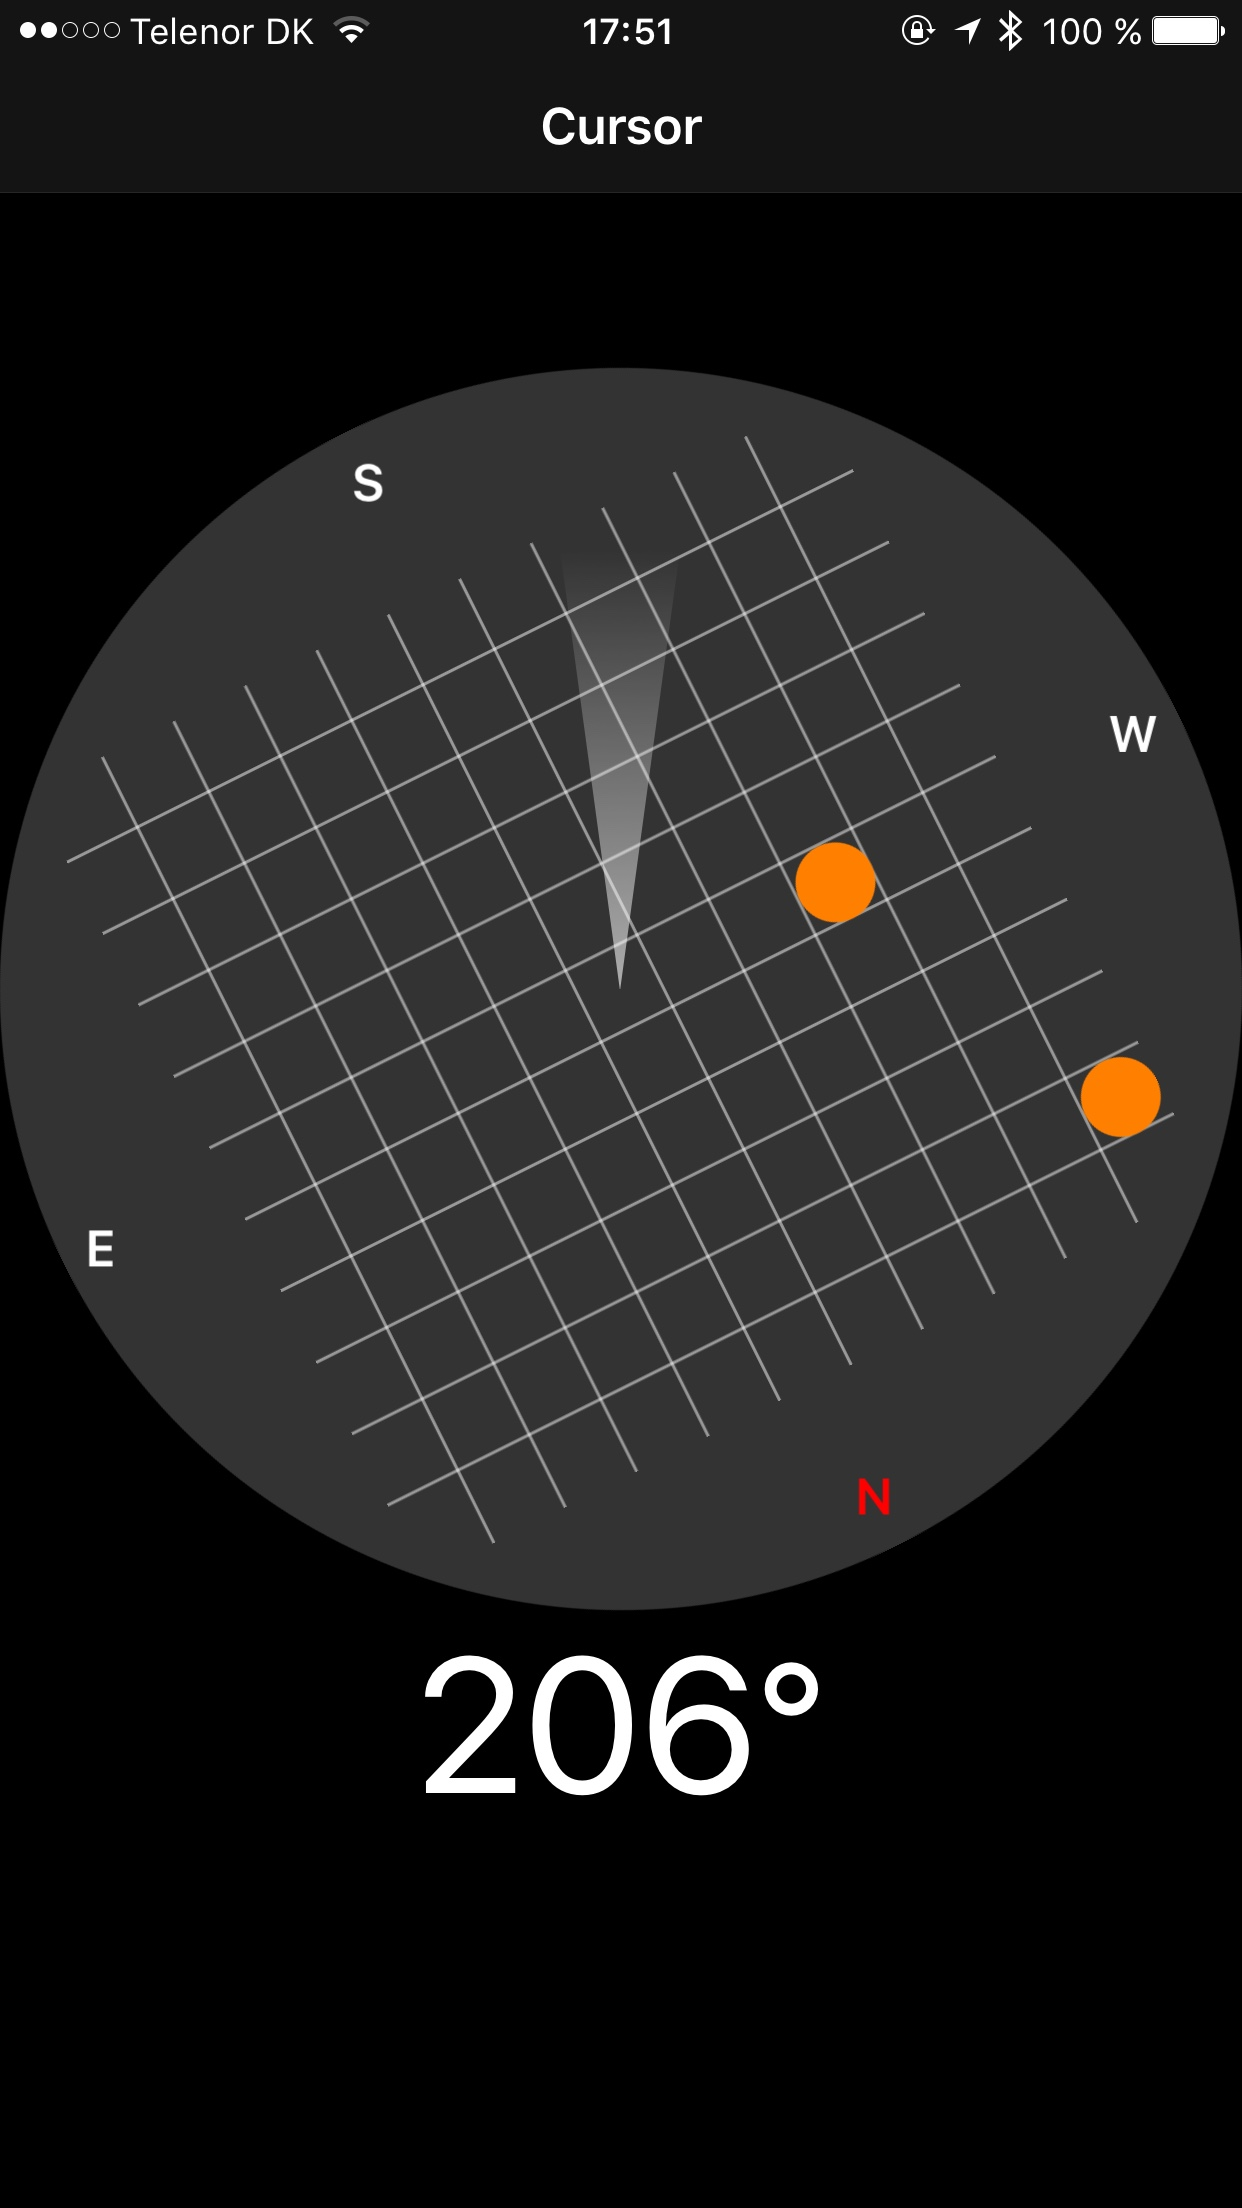
\includegraphics[width=0.3\textwidth]{images/Prototype2_iOS_1.png}
    }
    \subfloat{
        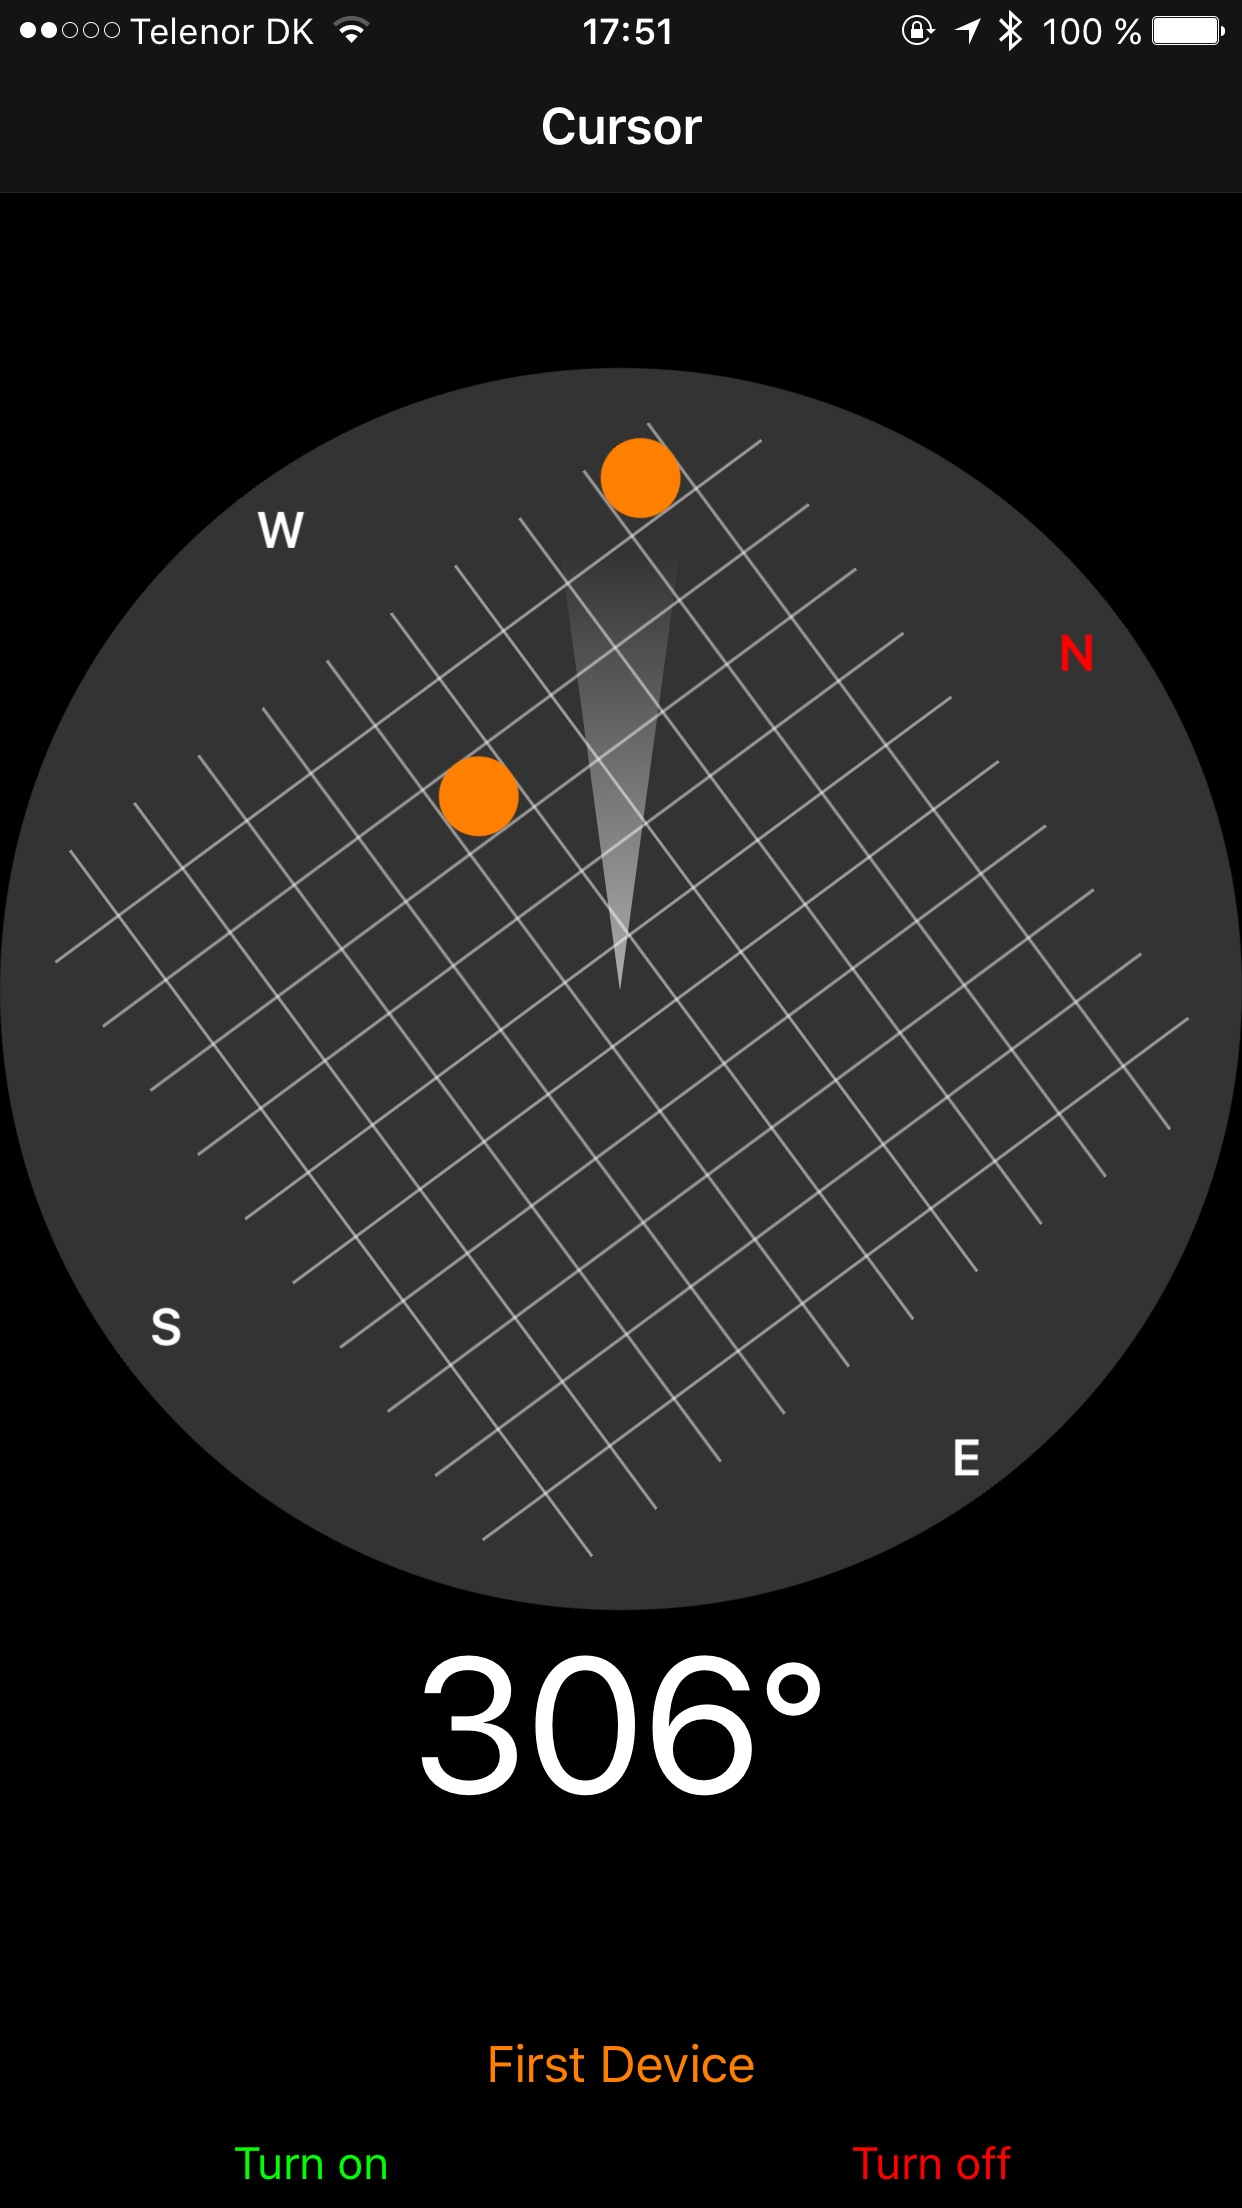
\includegraphics[width=0.3\textwidth]{images/Prototype2_iOS_2.png}
    }
    \caption{Screenshots of the second prototype application.}
    \label{fig:prototype2-app-screenshots}
\end{figure}

\begin{figure}
    \centering
    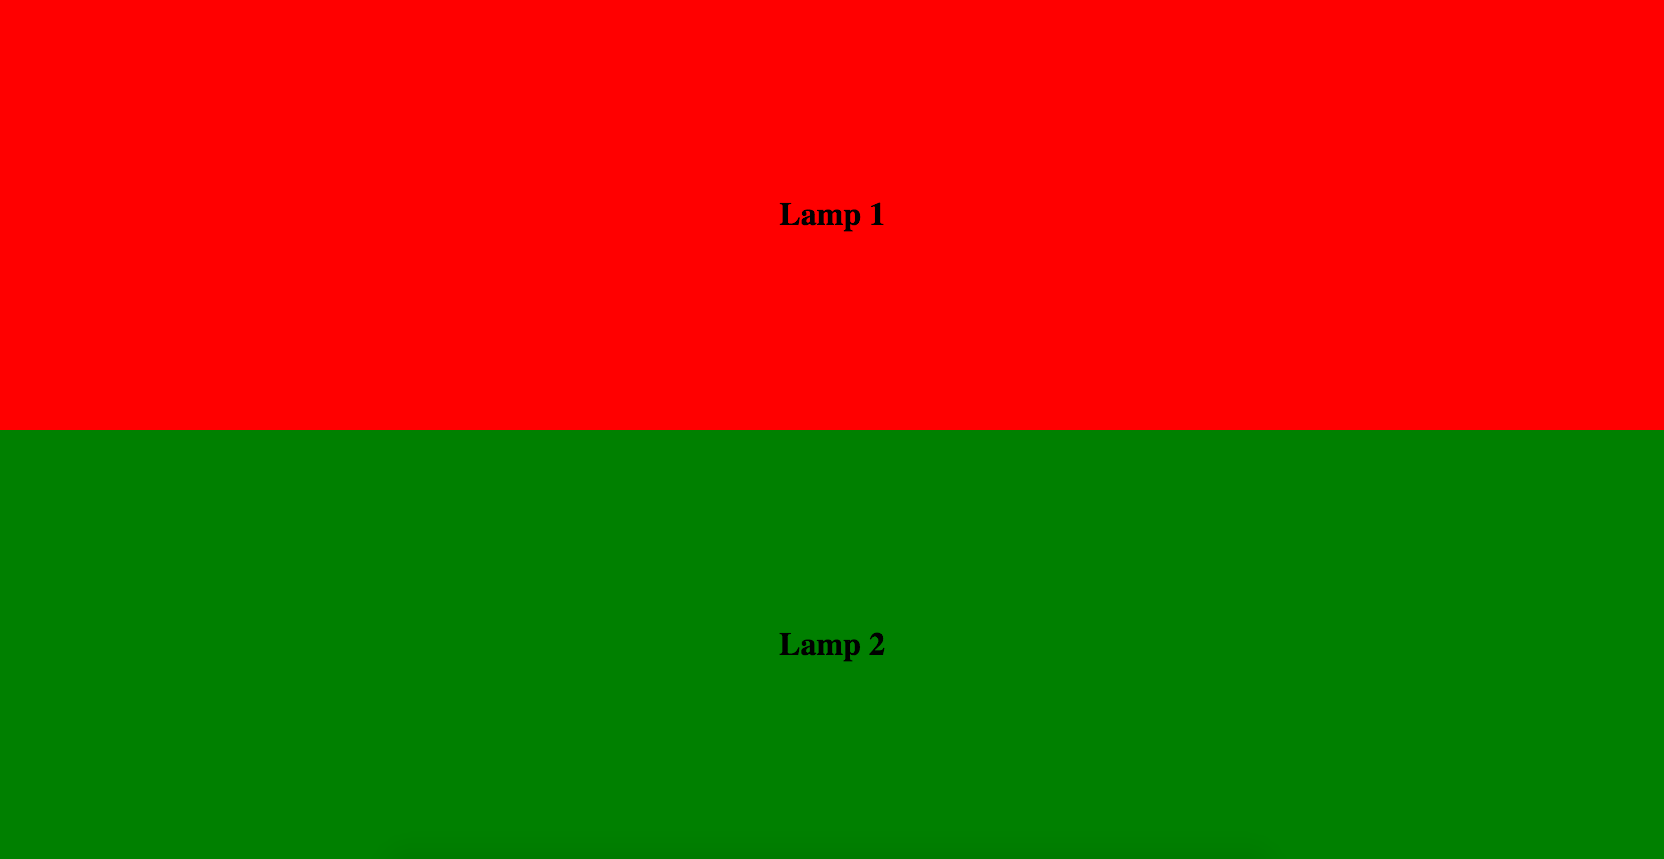
\includegraphics[scale=0.2]{images/Prototype2_Server.png}
    \caption[caption]{Screenshot of the server representing two lamps in the second prototype.\\\texttt{Green}: On, \texttt{Red}: Off}
    \label{fig:prototype2-server-screenshot}
\end{figure}
